\section{Task closure and the completion argument}\label{app:closure}
The proofs use ideal calibration tasks and their limiting readout weights, as specified in Sec.~2. Empty outcomes are omitted; a constant detector handles the associated trivial variables \cite[Sec.~6, footnote on p.~15]{cti}.

\subsection{Orthogonality closure}
Principle V and symmetry imply
\begin{equation}\label{eq:statewise}
 a\perp b\quad\Longleftrightarrow\quad
 \forall s\in a,\ t\in b:\ \{s\}\perp\{t\}.
\end{equation}
For the reverse direction, first use V to infer $\{s\}\perp b$ for each $s$, then use it again for $a$. Hence the bar operation is the polarity of a symmetric, irreflexive relation on states. It reverses inclusions, $a\subseteq\ddbar a$, and $\overline{\ddbar a}=\overline a$. Double bar is therefore extensive, monotone, and idempotent. Its closed sets are closed under intersections. Moreover,
\begin{equation}\label{eq:polarity}
 \overline{a\cup b}=\overline a\cap\overline b,
 \qquad \overline a\cap\cl(a)=\varnothing.
\end{equation}
The second equality follows because a state in the intersection would be orthogonal to itself. These facts prove the closure claims used in Eq.~\eqref{eq:completion}.

\subsection{Calibration on the closure of an attribute}
For any attribute $a$, the pair $\{\cl(a),\overline a\}$ is distinguishable by IV and V and has full domain. A measurer of it also measures $\{a,\overline a\}$. If a variable $X$ contains $a$, the Boolean measurer is a measurer of the binary coarse-graining that asks whether the input label is $a$. By VIII, all measurers of that coarse-graining are sharp on $\cl(a)$, since $\cl(a)\subseteq D_X$. This proves the closure property used for frequency windows and parity sectors.

A Boolean measurer can have sharp yes only on its closed yes attribute. Indeed, on a sharp-yes input $s$, that same measurer distinguishes $\{s\}$ from the no attribute $\overline a$. Thus $s\in\cl(a)$. Conversely, sharp yes on $\cl(a)$ is its calibration. No inference from the numerical condition $w=1$ to sharpness is involved.

\subsection{Full completion and comparison with the original contexts}
Let $x_i$ be the finite family of nonempty closed, pairwise distinguishable attributes in Theorem~\ref{thm:frequency}, and $r=\overline{\bigcup_i x_i}$. By Eq.~\eqref{eq:polarity}, the closure of their union with $r$ is $\Omega$. All members are distinguishable, including $r$ when nonempty. Let $D$ be the common discriminator from IV.

For fixed $i$, put $b_i=r\cup\bigcup_{j\ne i}x_j$. The coarse-graining $D_i$ is calibrated on $Y_i=\{x_i,b_i\}$, and $D_{Y_i}=\Omega$. Since $b_i\subseteq\overline{x_i}$, a Boolean measurer $T_i$ of $\{x_i,\overline{x_i}\}$ is also a measurer of $Y_i$. It is sharp no on $\overline{x_i}$. VIII, applied on $D_{Y_i}$, forces $D_i$ to be sharp no there too. It is already sharp yes on $x_i$. Thus $D_i$ is a Boolean measurer on all of $\Omega$.

Now let the original event arise as outcome $x_i$ of context $X_i$. Both $D_i$ and the original coarse detector measure
\begin{equation}\label{eq:comparison-variable}
 V_i=\left\{x_i,\ \bigcup_{x\in X_i,\ x\ne x_i}x\right\},
\end{equation}
whose domain equals $D_{X_i}$. Coverage puts the tested preparation in that domain. Equation~\eqref{eq:neutral} then compares the original event weight with the corresponding $D$ outcome. If a covered event is a coarse union rather than a closed outcome, replace that union by its closure; the preceding calibration property makes the replacement a closed event with the same detector on its legitimate domain.

When $\Delta>0$ in Eq.~\eqref{eq:converse}, $\sum_i w(D,i\mid\omega)\leq1$ gives
\begin{equation}\label{eq:excess-sum}
 \sum_i\bigl[w(e_i\mid\omega)-w(D,i\mid\omega)\bigr]\geq\Delta.
\end{equation}
At least one summand is at least $\Delta/m$. Combining it with Eq.~\eqref{eq:neutral} proves the stated lower bound for every $L$ and $f$.

\subsection{Approximation and task possibility}
For each $L$, the completion uses only finitely many discriminators, relabellings, and parallel networks. Under the task-accuracy convention, successively more accurate realizations retain all terminal records, including failure records, while uniform calibration errors vanish. Equations~\eqref{eq:mean}, \eqref{eq:ce}, and \eqref{eq:sum16} are finite inequalities in bounded record weights and persist in that limit. The frequency limit $L\to\infty$ is taken after fixing the finite-resolution task and its ideal readout weights; no unbounded constructor is claimed to be a finite apparatus.

\section{Frequency homogeneity and its quantum consistency}\label{app:frequency}
\subsection{A uniform partition is a homogeneous attribute}
Let $P_1,\ldots,P_k$ be a projective observable in finite dimension and let $A$ be an attribute of density operators. Define
\begin{equation}\label{eq:frequency-operator}
 F_{j,L}=\frac1L\sum_{\ell=1}^L P_j^{(\ell)}.
\end{equation}
A common frequency vector $f$ in mean square on all independent products from $A$ exists if and only if
\begin{equation}\label{eq:constant-frequencies}
 \Tr(\rho P_j)=f_j\quad\text{for every }\rho\in A\text{ and every }j.
\end{equation}
To prove this, set $p_{j,\ell}=\Tr(\rho_\ell P_j)$ and $\overline p_j=L^{-1}\sum_\ell p_{j,\ell}$. Direct expansion gives
\begin{equation}\label{eq:variance}
\begin{aligned}
 &\Tr\!\left[\left(\bigotimes_{\ell=1}^L\rho_\ell\right)(F_{j,L}-f_j I)^2\right]\\
 &\hspace{4mm}=(\overline p_j-f_j)^2+
 \frac1{L^2}\sum_{\ell=1}^L p_{j,\ell}(1-p_{j,\ell}).
\end{aligned}
\end{equation}
Taking every factor equal proves necessity. If Eq.~\eqref{eq:constant-frequencies} holds, the right side is at most $1/(4L)$ for every product, which proves sufficiency. For a closed support attribute consisting of all density operators on a subspace $S$, this is equivalent to
\begin{equation}\label{eq:compression}
 P_S P_j P_S=f_jP_S.
\end{equation}
The equivalence follows by evaluating all pure-state quadratic forms on $S$ and using polarization. This scalar-compression calculation is elementary; the analogous structure for a general error family appears in quantum error correction \cite{qec}.

\subsection{The exact one-sixteenth obstruction}
For $Z_+$, the probability or frequency parameter of outcome zero is $p\in[0,1/2]$. The quantum frequency identification here is the one explicitly made in Ref.~\cite[Sec.~5, E2, p.~28]{ctp}. For fixed mean $q=L^{-1}\sum_\ell p_\ell$, concavity of $p(1-p)$ bounds Eq.~\eqref{eq:variance} by
\begin{equation}\label{eq:qbound}
 (q-f)^2+\frac{q(1-q)}L,
\end{equation}
with equality when all $p_\ell=q$. This expression is convex in $q\in[0,1/2]$, including the affine case $L=1$. Its maximum is therefore
\begin{equation}\label{eq:endpointmax}
 \max\left\{f^2,\ (1/2-f)^2+\frac1{4L}\right\}.
\end{equation}
The minimum occurs when the two entries agree, at $f=(L+1)/(4L)$, proving Eq.~\eqref{eq:obstructionT1}.

The sign attributes $Z_\pm$ are closed because they are complete density-operator attributes on orthogonal subspaces. Applying $Z$ to the second qubit exchanges the signs. A controlled sign flip on a blank target copies the label; equivalently, conjugate a controlled-NOT by Hadamard gates on its source and target sign qubits. The unknown first qubit is untouched. Neither of the subspaces $\mathbb C^2\otimes\Span\{\ket\pm\}$ has a nonzero intersection with any eigenspace of $N_A+N_B$, but each has nonzero overlap with each eigenspace. This proves the generalized-mixture and information-variable assertions used in Sec.~6.

\begin{figure}[!htbp]
\centering
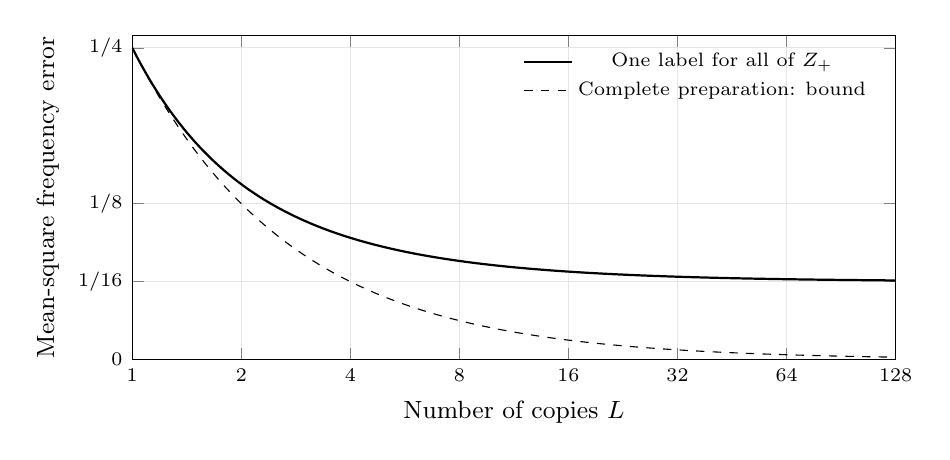
\begin{tikzpicture}
\begin{axis}[width=.93\columnwidth,height=5.7cm,
 xmode=log,log basis x=2,xmin=1,xmax=128,ymin=0,ymax=.26,
 xtick={1,2,4,8,16,32,64,128},xticklabels={1,2,4,8,16,32,64,128},
 ytick={0,.0625,.125,.25},yticklabels={$0$,$1/16$,$1/8$,$1/4$},
 xlabel={Number of copies $L$},ylabel={Mean-square frequency error},
 tick label style={font=\scriptsize},label style={font=\small},
 legend style={font=\scriptsize,at={(.98,.98)},anchor=north east,draw=none,fill=none},
 grid=major,grid style={gray!20}]
 \addplot[black,thick,domain=1:128,samples=180] {((x+1)/(4*x))^2};
 \addlegendentry{One label for all of $Z_+$}
 \addplot[black,dashed,domain=1:128,samples=180] {1/(4*x)};
 \addlegendentry{Complete preparation: bound}
\end{axis}
\end{tikzpicture}
\caption{A common frequency center for the unspecified first qubit leaves the exact error $((L+1)/(4L))^2$, approaching $1/16$. For one specified preparation, the variance about its own frequency is at most $1/(4L)$.}
\label{fig:frequency}
\end{figure}

\subsection{Complete quantum preparations satisfy H}
For a binary projective observable $\{P_0,P_1\}$, let $f=\Tr(\rho P_1)$ and let $Q$ be the spectral projector of $L^{-1}\sum_jP_1^{(j)}$ onto the window $[f-h,f+h]$. The input attribute in Eq.~\eqref{eq:window} is exactly the density operators supported on $Q$. From Eq.~\eqref{eq:variance} and the spectral inequality outside the window,
\begin{equation}\label{eq:quantum-tail}
 1-\Tr(Q\rho^{\otimes L})\leq\frac1{4Lh^2}.
\end{equation}
When $p=\Tr(Q\rho^{\otimes L})>0$, choose
\begin{equation}\label{eq:projected-state}
 \sigma=Q\rho^{\otimes L}Q/p.
\end{equation}
Purify $\rho^{\otimes L}$ to $\ket\psi$. Its normalized projection $\ket\phi=(Q\otimes I)\ket\psi/\sqrt p$ has squared overlap $p$. Diagonalizing the difference of their rank-one projectors in their two-dimensional span gives trace distance $\sqrt{1-p}$. Trace distance cannot increase under partial trace: in its variational expression as a supremum over effects, every effect on the reduced system is also an effect on the purification. Hence
\begin{equation}\label{eq:gentle}
 \frac12\|\rho^{\otimes L}-\sigma\|_1\leq\sqrt{1-p}.
\end{equation}
The quantum version of Eq.~\eqref{eq:metric} is bounded by trace distance, including finite ancillary readouts, again by the effect variational expression. Combining with Eq.~\eqref{eq:quantum-tail} proves Eq.~\eqref{eq:qH}; the bound one covers the remaining cases.

\section{The sixteen-set and five-set certificates}\label{app:certificates}
\subsection{Pairwise exclusivity and exact coverage}
Fix $t,c,d,k$ in Eq.~\eqref{eq:generator}, and write $k'=k\oplus1\oplus c\oplus d$. The eight fine events have Bob parity
\begin{equation}\label{eq:bob-parity}
 b\oplus b'=1\oplus\gamma_x\oplus xk\oplus(x\oplus t)k'.
\end{equation}
Its change between $x=0$ and $x=1$ is
\begin{equation}\label{eq:parity-change}
 c\oplus d\oplus k\oplus k'=1.
\end{equation}
Bob's two local settings are the same in both blocks. Two events from different blocks therefore disagree in at least one Bob output at the same setting. Events within a block differ in $a$ or $b$, also at the same setting. This proves all twenty-eight fine-event comparisons in each set. The remaining eight comparisons are supplied by the Alice parity opposite to $h_t^{cd}$. If that sector is empty, omit it and retain the same upper bound for at most nine events.

The last equation in Eq.~\eqref{eq:generator} gives
\begin{equation}\label{eq:same-status}
 a\oplus b\oplus xy=a'\oplus b'\oplus x'y'.
\end{equation}
Thus both component events win, or both lose. Conversely, consider any ordered pair satisfying Eq.~\eqref{eq:same-status}. Recover $t=x\oplus x'$, $k=y$, and $\gamma_x=1\oplus a\oplus a'$. The equation $c\oplus d=1\oplus y\oplus y'$ uniquely fixes the other $\gamma$ component. Equation~\eqref{eq:same-status} then fixes the displayed value of $b'$. The event pair occurs in exactly one generated set.

There are eight winning events and eight losing events in a single CHSH experiment. The sixteen sets therefore cover all $8^2+8^2=128$ ordered same-status pairs exactly once. Each parity outcome is included once for each $k$, hence twice. This proves Eq.~\eqref{eq:sum16} for arbitrary, possibly biased, Bell weights and certifies the construction underlying Ref.~\cite[Eq.~(10)]{cabello}.

\subsection{The residual polynomial}
Write $e=\eps_0+\eps_1$. The left side of Eq.~\eqref{eq:sum16} minus its right side is exactly
\begin{equation}\label{eq:residual-polynomial}
\begin{aligned}
 &\left(2+\frac B2\right)^2+\left(2-\frac B2\right)^2+4-2e\\
 &\quad-16-144\kappa=\frac{B^2-8-4e-288\kappa}{2}.
\end{aligned}
\end{equation}
For each $t$, the four displayed parity weights sum to $1-\eps_t$ by normalization of $\widehat J_t$, including the case of empty sectors. The eight parity weights occur twice in the sixteen event sums. This proves the residual coefficient four. The bound can also be combined with the algebraic inequality $|B|\leq4$, which follows from $|E_{xy}|\leq1$.

\subsection{The noisy-box rational certificates}
For Eq.~\eqref{eq:noisybox}, each winning event has weight $181/400$ and each losing event $19/400$. Direct summation gives normalized weights, uniform marginals independent of the remote setting, and
\begin{equation}\label{eq:box-values}
 B=\frac{81}{25},\qquad B^2-8=\frac{1561}{625}.
\end{equation}
For the five events of Eq.~\eqref{eq:five}, list their ten pairs in lexicographic order. A party witnessing equal setting and opposite output in each pair is respectively
\begin{equation}\label{eq:five-witnesses}
 3,\ 3,\ 2,\ 1,\ 2,\ 4,\ 1,\ 1,\ 4,\ 3.
\end{equation}
Each event wins both games. Equation~\eqref{eq:fiveexcess} follows by squaring its single-game weight and adding five times. Equations~\eqref{eq:converse} and \eqref{eq:kappabell} then give, without numerical approximation,
\begin{equation}\label{eq:kappa-thresholds}
 \kappa\geq\frac{761}{160000}
 \quad\text{or, with P,}\quad
 \kappa\geq\frac{1561}{180000}.
\end{equation}
The first inequality concerns the five-event completion; the second concerns the sixteen completions with P. Retaining the residual records instead gives Eq.~\eqref{eq:noisyresidual} from $B^2-8=1561/625$.

\section{Transporting closure and the T2 parity sectors}\label{app:transport}
The following lemma avoids assuming a reversible symmetry on the whole state space.

\begin{lemma}[Closure transport]\label{lem:transport}
Let $T$ be an available total transformation, including a fixed independent resource, and suppose $T(a)\subseteq b$. Then
\begin{equation}\label{eq:transport}
 T(\cl(a))\subseteq\cl(b).
\end{equation}
\end{lemma}
\begin{proof}
Follow $T$ by a Boolean measurer of $\{\cl(b),\overline b\}$. This circuit is sharp yes on $a$, so it is a measurer of the one-label calibration variable $\{a\}$. A constant-yes circuit measures the same variable and is sharp on $\cl(a)$. VIII therefore makes the composed circuit sharp yes throughout $\cl(a)$. A Boolean measurer has sharp yes only on $\cl(b)$, by Appendix~\ref{app:closure}. This proves Eq.~\eqref{eq:transport}. The one-label case uses the trivial constant-task convention.
\end{proof}

For the selected T2 sector, let $U_X^0=(x_0,x_0)\cup(x_1,x_1)$ and $U_X^1=(x_0,x_1)\cup(x_1,x_0)$; define $U_Y^0,U_Y^1$ analogously. R4 gives
\begin{equation}\label{eq:R4}
 q\subseteq\cl(U_X^0)\cap\cl(U_Y^0).
\end{equation}
The R2 task $T_X$ on the first copy maps each $U_X$ parity attribute into the opposite one while preserving both $U_Y$ parity labels. Similarly $T_Y$ exchanges the $Y$ parity and preserves the $X$ parity. These are simultaneous calibration requirements on the same implementations, as specified by R2. Lemma~\ref{lem:transport} extends these actions to the closed parity sectors.

It follows that $q,T_Xq,T_Yq,T_XT_Yq$ lie in the four sectors of Eq.~\eqref{eq:four}. Images of a nonempty physical attribute under a total available transformation are nonempty. Any two of these four attributes differ in an $X$ or $Y$ parity, and the corresponding parity measurer distinguishes them. Their enclosing intersections of closed sectors are also pairwise distinguishable and closed. IV supplies a common four-valued discriminator.

\subsection{Reversible transport and spectator-stable saturation}
If $G$ and $G^{-1}$ are available total transformations, applying Lemma~\ref{lem:transport} in both directions gives
\begin{equation}\label{eq:reversible-closure}
 G(\cl(a))=\cl(G(a)).
\end{equation}
The same maps preserve distinguishability: a discriminator can be preceded by the inverse transformation. Hence $G(\overline a)=\overline{G(a)}$. In particular, Eq.~\eqref{eq:interchange} on the second Alice copy maps the aligned product calibration unions to the crossed unions. Equation~\eqref{eq:reversible-closure} then maps each closed parity sector, its intersections, and its union closure as claimed in Theorem~\ref{thm:capacity}.

Here is the general saturation criterion. Let $K$ be an active composite with pairwise distinguishable closed attributes $h_1,\ldots,h_k$. Suppose their union contains a frame $\{f_1,\ldots,f_M\}$, each $f_i$ lying in one of the $h_j$. For a spectator $R$ with $\capn(R)=n$, assume the extended sectors contain every independent product $f_i\otimes z$, with $z$ a spectator attribute. If
\begin{equation}\label{eq:general-capacity}
 \capn(K\otimes R)\leq Mn,
\end{equation}
then the extended sectors have full domain.

To prove the claim, choose an $n$-element frame $\{z_j\}$. The $Mn$ product attributes $f_i\otimes z_j$ are pairwise distinguishable: a discriminator on $K$ separates different $i$, and one on $R$ separates different $j$. All products belong to the extended union. A nonempty bar of this union would supply a further distinguishable attribute, contradicting Eq.~\eqref{eq:general-capacity}. Its bar is therefore empty, which is exactly full double-bar coverage. If $M=\capn(K)$, the premise is the spectator-stable upper half of multiplicativity. The upper bound concerns the full composite, including correlated residual attributes, not just the independent calibration products.

\section{Quantum examples and comparisons}\label{app:quantum}
\subsection{Saturation and the parity domains}
Use $\ket\Phi=(\ket{00}+\ket{11})/\sqrt2$ in each Bell experiment. Alice measures $A_0=Z$, $A_1=X$, and Bob measures
\begin{equation}\label{eq:bob-observables}
 B_0=(Z+X)/\sqrt2,\qquad B_1=(Z-X)/\sqrt2.
\end{equation}
The correlators are $(1,1,1,-1)/\sqrt2$, obtained directly from $\langle Z\otimes Z\rangle=\langle X\otimes X\rangle=1$ and the vanishing cross correlators. Hence $B=2\sqrt2$.

On Alice's doubled subsystem the aligned parity operators are $Z\otimes Z$ and $X\otimes X$. The crossed operators are $Z\otimes X$ and $X\otimes Z$. In each pair the operators commute and square to the identity. Their four joint projectors are
\begin{equation}\label{eq:joint-projectors}
 \Pi^{cd}=\frac14(I+(-1)^cC_0)(I+(-1)^dC_1).
\end{equation}
They are orthogonal, have trace one, and sum to the identity. Thus their support attributes cover every two-qubit preparation, including arbitrary spectators. They realize P without imposing a two-coordinate local state space. The decoder in Fig.~\ref{fig:decoder} is $U=(H\otimes I)\operatorname{CNOT}$, where $H=(X+Z)/\sqrt2$. Direct conjugation gives
\begin{equation}\label{eq:decoder}
\begin{aligned}
 U^\dagger(Z\otimes I)U&=X\otimes X,\\
 U^\dagger(I\otimes Z)U&=Z\otimes Z.
\end{aligned}
\end{equation}
Also $HZH=X$ and $HXH=Z$, proving the setting-interchange property and the crossed decoder.

A quantum system of Hilbert-space dimension $D$ has information capacity $D$. Orthogonal pure states attain this value. Conversely, an effect that accepts every state of an attribute and rejects every state of another forces their support subspaces to be orthogonal. Indeed, $0\leq E\leq I$ and $\Tr(E\rho)=1$ imply that $E$ is the identity on $\supp\rho$, whereas $\Tr(E\sigma)=0$ implies it vanishes on $\supp\sigma$. Arbitrarily accurate discrimination gives the same conclusion by compactness of the effect interval. A finite frame thus occupies pairwise orthogonal nonzero subspaces, so its cardinality cannot exceed $D$. A spectator of dimension $D_R$ gives capacity $4D_R$ for Alice's doubled qubit and the spectator. This proves Eq.~\eqref{eq:capacity} for the full quantum composite, not just its product states.

The distinction between a binary sector and a binary-capacity carrier can be seen in a qutrit. Take $x_0,x_1$ to be the pure-state attributes of $\ket0,\ket1$, and $y_0,y_1$ those of $(\ket0\pm\ket1)/\sqrt2$. The selected two-attribute variables are legitimate information observables without being maximal \cite[Sec.~7, p.~19]{cti}. Extend the qubit flips and the Hadamard gate by the identity on $\ket2$. The generalized-mixture relations, simultaneous flip calibrations, intrinsic measurement attributes, and the state $\ket\Phi$ then satisfy R1--R4 within the two-level sector. The four aligned Bell sectors span only the four-dimensional space $\Span\{\ket0,\ket1\}^{\otimes2}$. Their residual support is five-dimensional and contains $\ket{22}$. Nevertheless, $\capn(S_A)=3$ and $\capn(S_A\otimes S_A)=9$. Thus T2 does not imply the full-carrier bound in Eq.~\eqref{eq:capacity}, even with a trivial spectator. Preparations covered by the selected binary local observables still lie in the two-level sector and satisfy P in this example.

\subsection{Parity coverage is not automatic for arbitrary quantum settings}
Let $A_0=Z$ and $A_1=(3Z+4X)/5$. They are binary projective observables because $A_1^2=I$. Their aligned parity operators satisfy
\begin{equation}\label{eq:tilted-commutator}
 [A_0\otimes A_0,A_1\otimes A_1]
 =\frac{24i}{25}(I\otimes Y+Y\otimes I),
\end{equation}
whose operator norm is $48/25$. The norm follows from the eigenvalues $2,0,0,-2$ of the parenthesized operator. If their common eigenspaces spanned the whole space, a basis of common eigenvectors would make the operators commute. Equation~\eqref{eq:tilted-commutator} rules that out. Thus their common parity-sector variable does not have full domain, although it can still cover particular preparations.

\subsection{Nonperturbation need not be minimal disturbance}
On two qubits, consider the instrument
\begin{equation}\label{eq:reset}
 \mathcal M_i(\rho)=\ket{i0}\bra{i0}\,
 \Tr[(\ket i\bra i\otimes I)\rho],\quad i=0,1.
\end{equation}
It is completely positive, and its sum preserves trace. It reads the first-qubit label and leaves that label unchanged, so it is nonperturbing on its calibrated attributes and repeatable. The compatible readout $Q=I\otimes\ket1\bra1$ has weight one on $\ket{01}\bra{01}$ and zero after the instrument. The disturbance is exactly one. It therefore fails the minimal-disturbance condition of Ref.~\cite[Eq.~(4)]{sharp}. The same first-qubit effects do admit a L\"uders implementation; this example separates instrument conditions, not their possible statistics.

\subsection{The almost-quantum comparison}
The representation in Ref.~\cite[Definition 1 and Sec.~6]{aq} assigns projectors to local outcomes and a state on which the relevant products have the required order independence. For binary outcomes put $A_x=P_0^x-P_1^x$ and $B_y=Q_0^y-Q_1^y$. On that state $\ket\psi$, define unit vectors $u_x=A_x\ket\psi$ and $v_y=B_y\ket\psi$. Their real inner products are the correlators. Therefore
\begin{equation}\label{eq:gram-bound}
\begin{aligned}
 |B|&\leq\|v_0+v_1\|+\|v_0-v_1\|\\
 &\leq\sqrt{2\bigl(\|v_0+v_1\|^2+\|v_0-v_1\|^2\bigr)}
 =2\sqrt2.
\end{aligned}
\end{equation}
This is the standard Gram-vector bound for that representation.

\section{Readable labels and the published hypersignaling witness}\label{app:hs}
This appendix separates two dimension notions using the HS model of Ref.~\cite[Eq.~(4) and Supplemental Material]{hs}. The model and the seven-input witness are prior work. We give an analytic proof of its readable-alphabet bound and evaluate the witness exactly.

\subsection{Two locally readable labels, four jointly}
For this comparison only, let $\drec(S)$ be the maximum number of prepared states distinguished by one measurement. Under IV and preparation access it equals $\capn(S)$, but we will not impose IV on the comparison model.

The elementary normalized state space is the convex hull of
\begin{equation}\label{eq:hs-states}
\begin{aligned}
 v_0&=(1,0,1)^T,&v_1&=(0,1,1)^T,\\
 v_2&=(-1,0,1)^T,&v_3&=(0,-1,1)^T.
\end{aligned}
\end{equation}
The unit effect is $u=(0,0,1)^T$, and all positive effects are allowed. The four extreme rays of the effect cone are
\begin{equation}\label{eq:hs-effects}
\begin{aligned}
 e_0&=(1,1,1)^T,&e_1&=(-1,1,1)^T,\\
 e_2&=(-1,-1,1)^T,&e_3&=(1,-1,1)^T.
\end{aligned}
\end{equation}
These rays follow by imposing nonnegative evaluation on the four displayed vertices. Any finite measurement can be refined into effects proportional to $e_i$. Normalization forces their total coefficients to have the form $(a,b,a,b)$ with $2a+2b=1$. Thus every measurement is a mixture of the two binary measurements $\{e_0/2,e_2/2\}$ and $\{e_1/2,e_3/2\}$, followed by classical postprocessing. Sending the binary outcome simulates any such readout with shared randomness. Hence $s(S)=2$, with equality because $v_0,v_2$ are perfectly distinguishable.

Let $c=(0,0,1)^T$ denote the center state. Since $2c-v_i$ is a normalized state, any effect $f$ satisfies $f(v_i)\leq2f(c)$, and convexity extends this to every normalized state. If $N$ states are read with error at most $\xi$, summing over their respective effects gives $N(1-\xi)\leq2$. Consequently $\drec(S)=2$.

The bipartite normalized states are all convex mixtures of $v_i\otimes v_j$, again with all positive effects. Cone positivity gives
\begin{equation}\label{eq:hs-cone}
\begin{aligned}
 4c\otimes c-v_i\otimes v_j
 &=(2c-v_i)\otimes2c\\
 &\quad+v_i\otimes(2c-v_j)\geq0.
\end{aligned}
\end{equation}
Applying the same bound to every outcome of a common measurement gives $N(1-\xi)\leq4$. The products of $v_0,v_2$ form a four-label readable frame, so
\begin{equation}\label{eq:hs-readable}
 \drec(S\otimes S)=4=\drec(S)^2.
\end{equation}
This proof includes arbitrary mixed preparations and arbitrarily accurate discrimination limits.

Each pair of different elementary vertices can nevertheless be distinguished by some binary measurement: evaluation of the $e_i/2$ gives an opposite sharp pair. Since no one measurement distinguishes all four, principle IV fails. The comparison therefore does not decide whether the two dimension notions can differ under every constructor premise.

\subsection{A channel that needs more than four classical symbols}
Represent the product state $v_i\otimes v_j$ by the matrix $\Omega_{4i+j}=v_iv_j^T$, and put $E_{4i+j}=e_ie_j^T$, with $i,j\in\{0,1,2,3\}$. Matrix evaluation is $\Tr(\Omega^TE)$. Define
\begin{equation}\label{eq:e23}
 E_{23}=\begin{pmatrix}-1&-1&0\\1&-1&0\\0&0&1\end{pmatrix}.
\end{equation}
The subscript follows the source's enumeration. The seven measurement effects are
\begin{equation}\label{eq:hs-measurement}
 \frac18 E_0,\ \frac18 E_1,\ \frac18 E_6,\ \frac18 E_8,
 \ \frac18 E_{10},\ \frac18 E_{15},\ \frac14 E_{23}.
\end{equation}
Their sum is $uu^T$. The first six terms are positive products. Since the planar parts of $v_i,v_j$ are signed coordinate vectors, $E_{23}$ evaluates to either zero or two on every product vertex. Convexity proves validity on the entire declared state space.

For preparations $(\Omega_0,\Omega_2,\Omega_6,\Omega_7,\Omega_{12},\Omega_{13},\Omega_{15})$, respectively, the two nonzero output positions in each row are
\begin{equation}\label{eq:hs-channel}
\begin{gathered}
 (1,6),\ (2,7),\ (2,3),\ (3,7),\\
 (4,6),\ (4,7),\ (5,6).
\end{gathered}
\end{equation}
Each displayed position has weight $1/2$, defining a channel $\Xi$. This is the channel in Ref.~\cite[Eq.~(4)]{hs}. Its payoff matrix is
\begin{equation}\label{eq:payoff}
 \Gamma=\frac1{21}\begin{pmatrix}
 2&0&0&0&0&1&0\\
 0&2&0&0&0&0&2\\
 0&2&2&0&0&0&0\\
 0&0&2&0&0&0&2\\
 0&0&0&1&0&1&0\\
 0&0&0&1&0&0&0\\
 0&0&0&0&2&1&0
 \end{pmatrix}.
\end{equation}
Direct substitution gives $\sum_{ij}\Gamma_{ij}\Xi_{ij}=1/2$.

A deterministic four-symbol simulation uses a set $J$ of at most four output columns, so its best payoff is $\sum_i\max_{j\in J}\Gamma_{ij}$. Nonnegative entries let us enlarge $J$ to four columns. Let $k$ count the selected columns from $\{2,3,7\}$, let $l$ count those from $\{1,4,5\}$, and let $b$ indicate whether column six is selected. Then $k+l+b=4$. The unscaled row-maximum sum is exactly
\begin{equation}\label{eq:hs-score}
\begin{gathered}
 r(k)+2l+b(3-l),\\
 (r(0),r(1),r(2),r(3))=(0,4,6,6).
\end{gathered}
\end{equation}
For $b=0$, the pair $(k,l)$ is $(1,3),(2,2)$, or $(3,1)$, giving respective scores $10,10$, and $8$. For $b=1$, it is $(0,3),(1,2),(2,1)$, or $(3,0)$, giving $6,9,10$, and $9$. Thus the maximum is $10/21$. Shared randomness cannot increase a linear payoff. We have proved the exact separation
\begin{equation}\label{eq:hs-gap}
 \sum_{ij}\Gamma_{ij}\Xi_{ij}
 -\max_{\text{four symbols}}\sum_{ij}\Gamma_{ij}p(j\mid i)
 =\frac1{42}.
\end{equation}
It follows that $s(S\otimes S)>4=s(S)^2$, despite Eq.~\eqref{eq:hs-readable}. The certificate program also evaluates all thirty-five four-column choices and reconstructs the channel directly from Eq.~\eqref{eq:hs-measurement}.

\paragraph{Acknowledgments.}
AI assistance supported literature review, proof exploration, and preparation of the manuscript and verification code. The author is responsible for the results.
